\documentclass[aspectratio=169,11pt]{beamer}
\usetheme{default}
\usecolortheme{default}

\setbeamertemplate{navigation symbols}{}
\setbeamertemplate{footline}[frame number]

\usepackage{amsmath}
\usepackage{booktabs}
\usepackage{graphicx}

% Small citation macro
\newcommand{\citeslide}[1]{\hfill{\footnotesize [#1]}}

\title{Trainable Chemical Reaction Networks}
\subtitle{First Results: A Recurrent Neural CRN Solving XOR}
\author{Srivijayesh Venugopal}
\date{Cranfield IRP 2025-26}

\begin{document}

% ---------------------------------------------------------------------
\begin{frame}
\titlepage
\end{frame}

% ---------------------------------------------------------------------
\begin{frame}{Where we are}

We have pivoted from acoustic wave computing to chemical reaction networks (CRNs).

\vspace{0.3cm}
This deck shows the first numerical result:
\begin{itemize}
    \item a small recurrent CRN,
    \item trained by optimizing rate constants,
    \item that learns the XOR function.
\end{itemize}

\vspace{0.3cm}
This is the well-mixed, deterministic starting point before adding spatial reaction-diffusion.

\end{frame}

% ---------------------------------------------------------------------
\begin{frame}{Why CRNs fit a computational physics thesis}

The forward model is a system of ODEs:
\begin{equation*}
    \frac{d\mathbf{c}}{dt} = \mathbf{S}\,\mathbf{r}(\mathbf{c}; \mathbf{k})
\end{equation*}

\vspace{0.2cm}
where:
\begin{itemize}
    \item $\mathbf{c}$ = species concentration vector,
    \item $\mathbf{S}$ = stoichiometry matrix,
    \item $\mathbf{r}$ = mass-action rate vector,
    \item $\mathbf{k}$ = trainable rate constants.
\end{itemize}

\vspace{0.3cm}
Add diffusion and the model becomes the reaction-diffusion PDE:
\begin{equation*}
    \frac{\partial \mathbf{c}}{\partial t} = \mathbf{D}\nabla^2 \mathbf{c} + \mathbf{S}\,\mathbf{r}(\mathbf{c}; \mathbf{k})
\end{equation*}

\vspace{0.2cm}
\centering
\textbf{This is standard reactive transport. The program is in the chemistry and geometry.}

\end{frame}

% ---------------------------------------------------------------------
\begin{frame}{Core idea: a CRN as a trainable dynamical system}

A neural network maps inputs to outputs through layers.

\vspace{0.3cm}
A CRN does the same thing, but in continuous time:
\begin{itemize}
    \item inputs = initial concentrations,
    \item hidden computation = coupled reactions,
    \item output = a concentration at a later time.
\end{itemize}

\vspace{0.3cm}
Training means adjusting reaction rates so the trajectory ends in the right place.

\end{frame}

% ---------------------------------------------------------------------
\begin{frame}{Dack's RNCRN architecture}

Two groups of species \citeslide{Dack et al., 2024}:
\begin{itemize}
    \item \textbf{Executive species} $X_i$: the variables we read and write.
    \item \textbf{Chemical perceptrons} $Y_j$: fast auxiliary species that create nonlinearity.
\end{itemize}

\vspace{0.3cm}
Mass-action dynamics:
\begin{align*}
    \frac{dX_i}{dt} &= \beta_i + X_i \sum_j \alpha_{ij} Y_j \\[0.5em]
    \frac{dY_j}{dt} &= \frac{1}{\mu} \left[ \gamma + \theta_j Y_j + Y_j \sum_i \omega_{ji} X_i - Y_j^2 \right]
\end{align*}

\vspace{0.2cm}
$\mu \ll 1$ makes perceptrons much faster than executives.

\end{frame}

% ---------------------------------------------------------------------
\begin{frame}{The perceptrons act as a smooth ReLU}

For small $\mu$, each $Y_j$ quickly reaches its steady state:
\begin{equation*}
    Y_j^* = \sigma_\gamma\left( \sum_i \omega_{ji} X_i + \theta_j \right)
\end{equation*}

\vspace{0.2cm}
The chemical activation is:
\begin{equation*}
    \sigma_\gamma(z) = \frac{1}{2}\left( z + \sqrt{z^2 + 4\gamma} \right)
\end{equation*}

\vspace{0.2cm}
\begin{itemize}
    \item $z \gg 0$: $\sigma_\gamma(z) \approx z$.
    \item $z \ll 0$: $\sigma_\gamma(z) \approx 0$.
    \item $\gamma$ rounds the ReLU corner.
\end{itemize}

\vspace{0.2cm}
\centering
\textbf{So the fast perceptrons form a hidden layer of smooth ReLU neurons.}

\end{frame}

% ---------------------------------------------------------------------
\begin{frame}{Feedforward vs recurrent CRN}

\begin{table}
\centering
\begin{tabular}{lcc}
\toprule
\textbf{Feature} & \textbf{Feedforward} & \textbf{Recurrent} \\
\midrule
Perceptron sees & $X_1, X_2$ & $X_1, X_2, X_3$ \\
Output feeds back & no & yes \\
Dynamics & simple steady state & switching, amplification \\
Training & easy & needs bounding \\
Closer to Dack's original construction & no & yes \\
\bottomrule
\end{tabular}
\end{table}

\end{frame}

% ---------------------------------------------------------------------
\begin{frame}{XOR benchmark}

XOR is the classic nonlinearly separable test:

\vspace{0.3cm}
\begin{table}
\centering
\begin{tabular}{cc|c}
\toprule
$X_1$ & $X_2$ & \textbf{target} $X_3$ \\
\midrule
0 & 0 & 0 \\
0 & 1 & 1 \\
1 & 0 & 1 \\
1 & 1 & 0 \\
\bottomrule
\end{tabular}
\end{table}

\vspace{0.3cm}
Network layout:
\begin{itemize}
    \item 2 pinned inputs: $X_1$, $X_2$.
    \item 1 output: $X_3$.
    \item 4 chemical perceptrons: $Y_1$ to $Y_4$.
    \item Trainable: $\alpha$, $\omega$, $\theta$, $\beta_3$.
\end{itemize}

\end{frame}

% ---------------------------------------------------------------------
\begin{frame}{Numerical method}

\begin{enumerate}
    \item Integrate the ODE system with \texttt{scipy.integrate.solve\_ivp}.
    \item Define loss = mean squared error between $X_3(T)$ and target XOR values.
    \item Optimize rate constants with L-BFGS-B.
    \item Restart from several random initializations to avoid poor local minima.
\end{enumerate}

\vspace{0.3cm}
For the recurrent version, the output $X_3$ is bounded into $(0,1)$ with a sigmoid transform to prevent runaway feedback during training.

\end{frame}

% ---------------------------------------------------------------------
\begin{frame}{Result: recurrent RNCRN solving XOR}

\centering
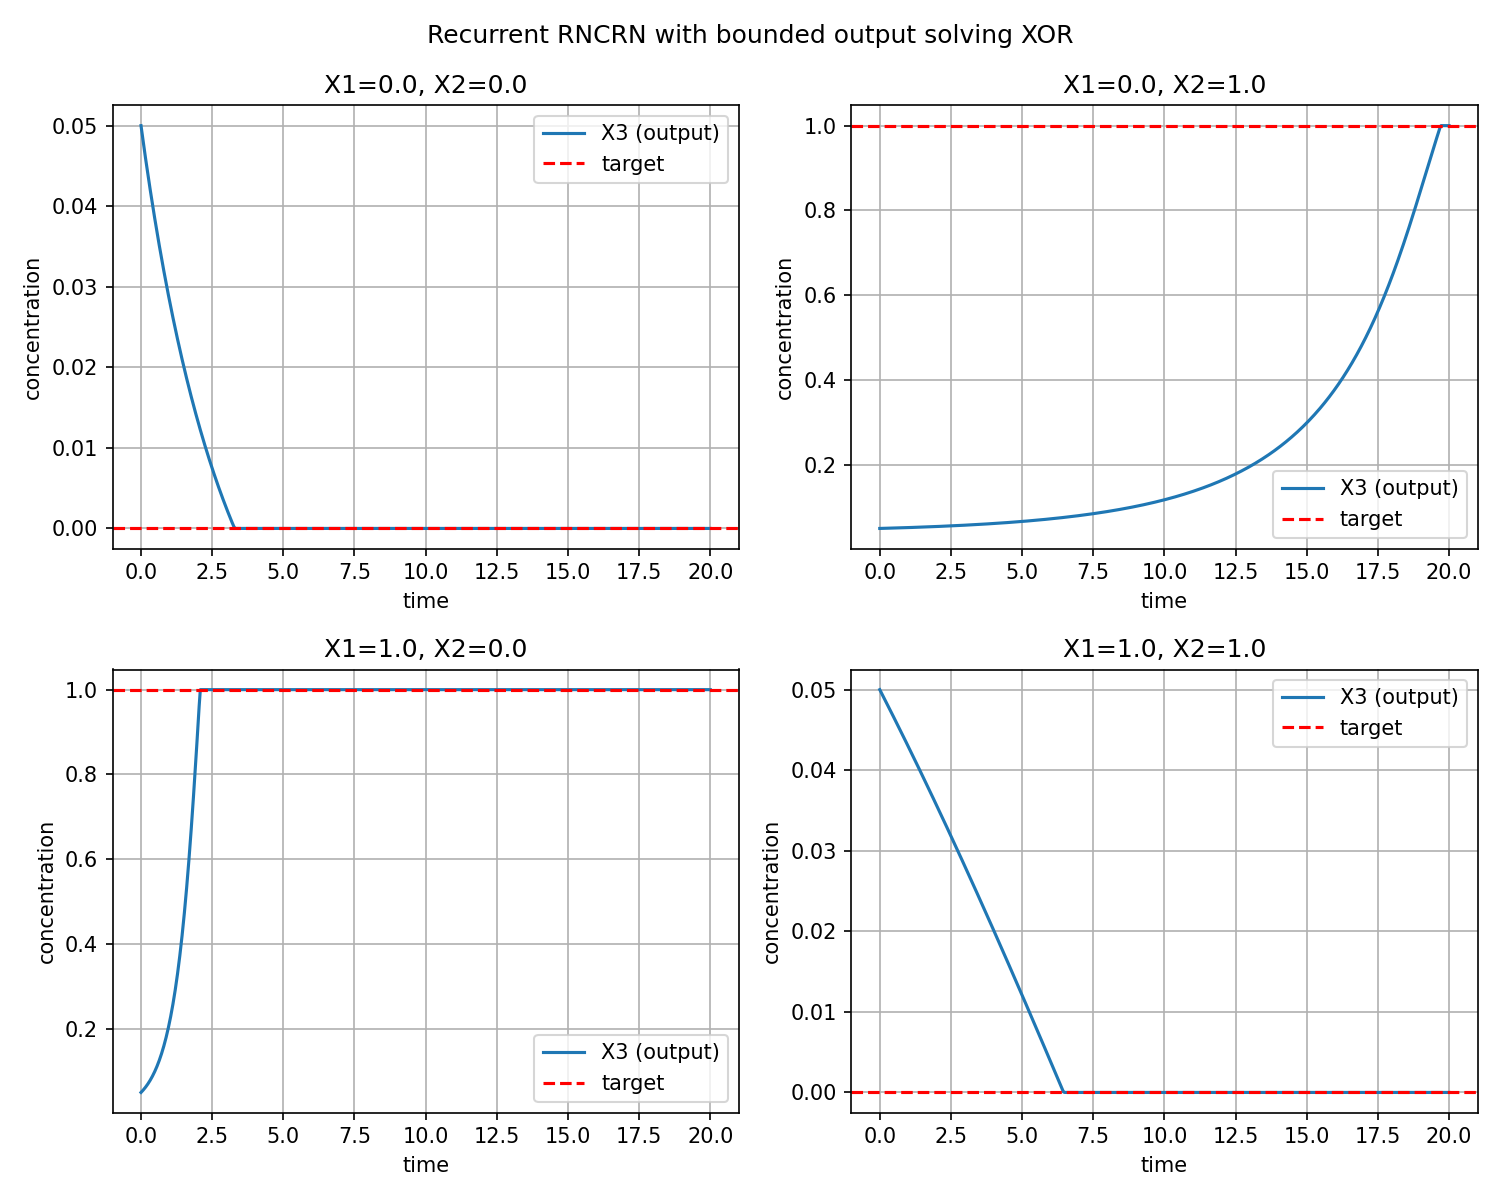
\includegraphics[width=0.65\textwidth]{../Analysis/dack_rncrn_xor_recurrent_bounded_results.png}

\vspace{0.3cm}
The output $X_3(t)$ converges to the correct XOR value for all four inputs.

\end{frame}

% ---------------------------------------------------------------------
\begin{frame}{Truth table}

\begin{table}
\centering
\begin{tabular}{cc|cc}
\toprule
$X_1$ & $X_2$ & \textbf{target} & \textbf{predicted $X_3$} \\
\midrule
0 & 0 & 0 & 0.0000 \\
0 & 1 & 1 & 1.0000 \\
1 & 0 & 1 & 1.0000 \\
1 & 1 & 0 & 0.0000 \\
\bottomrule
\end{tabular}
\end{table}

\vspace{0.3cm}
\centering
\textbf{Loss $\approx 0$ over the four cases.}

\end{frame}

% ---------------------------------------------------------------------
\begin{frame}{What this shows and what it does not}

\textbf{Shows:}
\begin{itemize}
    \item A CRN with trainable rate constants can learn a nonlinear Boolean function.
    \item the quasi-steady-state approximation of the fast perceptrons is used. 
    \item The Dack RNCRN architecture works in practice, not just in theory \citeslide{Dack et al., 2024}.
\end{itemize}

\vspace{0.3cm}
\textbf{Does not show:}
\begin{itemize}
    \item Stochastic robustness at finite molecule counts.
    \item Spatial reaction-diffusion behavior.
    \item Chemical realizability of the learned rates.
\end{itemize}

\end{frame}

% ---------------------------------------------------------------------
\begin{frame}{Next steps}

\begin{enumerate}
    \item \textbf{Stochastic study:} run simulations with finite copy numbers and quantify XOR accuracy.
    \item \textbf{Regularization:} constrain rate constants to chemically plausible magnitudes.
    \item \textbf{Spatial extension:} add diffusion on a 1D/2D grid and train a reaction-diffusion classifier.
    \item \textbf{Gating:} use a control species to switch the same network between two functions.
    \item \textbf{Baseline comparison:} compare energy, delay, and accuracy against a digital implementation.
\end{enumerate}

\end{frame}

% ---------------------------------------------------------------------
\begin{frame}{Conclusion}

\begin{itemize}
    \item We now have a working trainable CRN baseline.
    \item A recurrent neural CRN can be optimized to solve XOR.
    \item The model is mathematically clean and extensible to reaction-diffusion.
    \item Next steps: stochastic robustness and a spatial classifier.
\end{itemize}

\end{frame}

% ---------------------------------------------------------------------
\begin{frame}{References}

{\footnotesize
\begin{enumerate}
    \item A. Dack, B. Qureshi, T. E. Ouldridge, \u0026 T. Plesa. Recurrent neural chemical reaction networks that approximate arbitrary dynamics. \textit{Cell Systems}, 2026. arXiv:2406.03456.

    \item M. G. Baltussen \textit{et al.} Chemical reservoir computation in a self-organizing reaction network. \textit{Nature} 631, 549-555 (2024).

    \item K. M. Cherry \u0026 L. Qian. Supervised learning in DNA neural networks. \textit{Nature} 645, 639-647 (2025).

    \item L. Qian, E. Winfree, \u0026 J. Bruck. Neural network computation with DNA strand displacement cascades. \textit{Nature} 475, 368-372 (2011).

    \item S. Okumura \textit{et al.} Nonlinear decision-making with enzymatic neural networks. \textit{Nature} 610, 496-501 (2022).

    \item M. Stern \u0026 A. Murugan. Learning without neurons in physical systems. \textit{Annu. Rev. Condens. Matter Phys.} 14, 417-441 (2023).

    \item A. Adamatzky \u0026 B. De Lacy Costello. Experimental logical gates in a reaction-diffusion medium. \textit{Phys. Rev. E} 66, 046112 (2002).
\end{enumerate}
}

\end{frame}

\end{document}
